\section{Muhammad Fahmi(1174021)}
\subsection{PYSHP Reader}
\begin{enumerate}
    \item Buatlah Script Python dan jelaskan perbaris
    \lstinputlisting[firstline=1, lastline=4]{src/1174021/3/read.py}
    \hfill\break
    \begin{itemize}
        \item Baris pertama Digunakan untuk memanggil library SHP
        \item Digunakan untuk melakukan membaca file shp
        \item Menampilkan apa yang telah dipanggil pada variabel sf
    \end{itemize}
    \hfill\break
    \begin{figure}[H]
		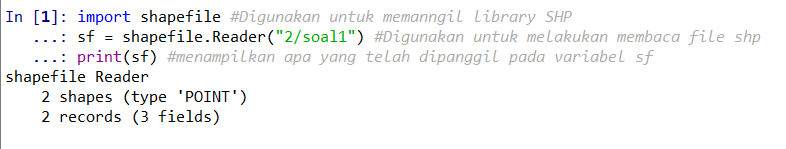
\includegraphics[width=4cm]{figures/1174021/3/soal1.PNG}
		\centering
		\caption{Hasil Read File SHP Soal 1}
    \end{figure}
    
    \item Buatlah Script Python dan jelaskan perbaris
    \lstinputlisting[firstline=6, lastline=9]{src/1174021/3/read.py}
    \hfill\break
    \begin{itemize}
        \item Baris pertama Digunakan untuk memanggil library SHP
        \item Digunakan untuk melakukan membaca file shp
        \item Berfungsi untuk mengetahui Type dari file SHP yang dibaca
    \end{itemize}
    \hfill\break
    \begin{figure}[H]
		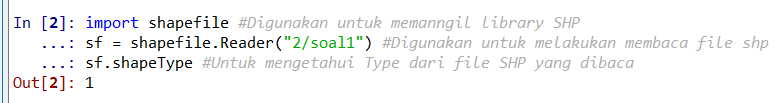
\includegraphics[width=4cm]{figures/1174021/3/soal2.PNG}
		\centering
		\caption{Hasil Read File SHP Soal 2}
    \end{figure}

    \item Buatlah Script Python dan jelaskan perbaris
    \lstinputlisting[firstline=11, lastline=14]{src/1174021/3/read.py}
    \hfill\break
    \begin{itemize}
        \item Baris pertama Digunakan untuk memanggil library SHP
        \item Digunakan untuk melakukan membaca file shp
        \item Berfungsi untuk mengetahui garis tepi pada file shp tersebut
    \end{itemize}
    \hfill\break
    \begin{figure}[H]
		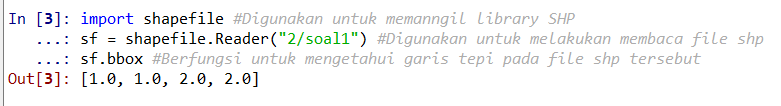
\includegraphics[width=4cm]{figures/1174021/3/soal3.PNG}
		\centering
		\caption{Hasil Read File SHP Soal 3}
    \end{figure}
    
    \item Buatlah Script Python dan jelaskan perbaris
    \lstinputlisting[firstline=16, lastline=20]{src/1174021/3/read.py}
    \hfill\break
     \begin{itemize}
        \item Baris pertama Digunakan untuk memanggil library SHP
        \item Digunakan untuk melakukan membaca file shp
        \item Berfungsi untuk membaca jumlah data yang ada di file shp tersebut
        \item Berfungsi untuk menampilkan jumlah data dari file shp tersebut
    \end{itemize}
    \hfill\break
    \begin{figure}[H]
		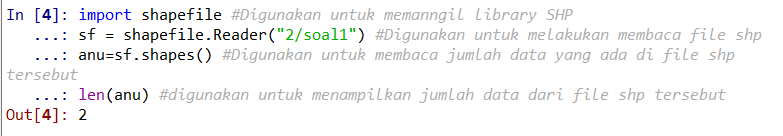
\includegraphics[width=4cm]{figures/1174021/3/soal4.PNG}
		\centering
		\caption{Hasil Read File SHP Soal 4}
    \end{figure}
    
    \item Buatlah Script Python dan jelaskan perbaris
    \lstinputlisting[firstline=22, lastline=27]{src/1174021/3/read.py}
    \hfill\break
     \begin{itemize}
        \item Baris pertama Digunakan untuk memanggil library SHP
        \item Digunakan untuk melakukan membaca file shp
        \item Berfungsi untuk membaca jumlah data yang ada di file shp tersebut
        \item Digunakan mengetahui object yang digunakan
        \item Digunakan untuk mengetahui object yang digunakan berdasarkan nomor index 0
    \end{itemize}
    \hfill\break
    \begin{figure}[H]
		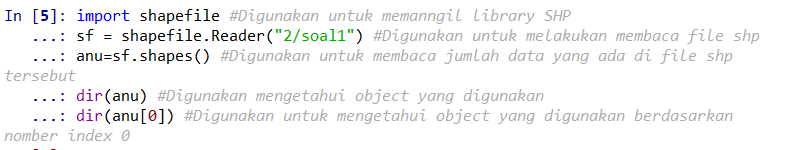
\includegraphics[width=4cm]{figures/1174021/3/soal5_1.PNG}
		\centering
		\caption{Hasil Read File SHP Soal 5}
    \end{figure}
    \hfill\break
    \begin{figure}[H]
		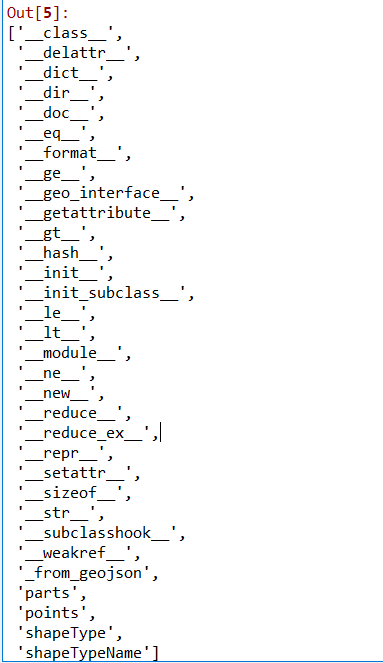
\includegraphics[width=4cm]{figures/1174021/3/soal5_2.PNG}
		\centering
		\caption{Hasil Read File SHP Soal 5}
    \end{figure}
    
    \item Buatlah Script Python dan jelaskan perbaris
    \lstinputlisting[firstline=29, lastline=33]{src/1174021/3/read.py}
    \hfill\break
    \begin{itemize}
        \item Baris pertama Digunakan untuk memanggil library SHP
        \item Digunakan untuk melakukan membaca file shp
        \item Berfungsi untuk membaca jumlah data yang ada di file shp tersebut
        \item Digunakan untuk membaca shape type yang digunakan pada index ke 0
    \end{itemize}
    \hfill\break
    \begin{figure}[H]
		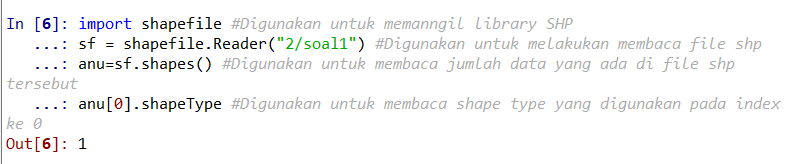
\includegraphics[width=4cm]{figures/1174021/3/soal6.PNG}
		\centering
		\caption{Hasil Read File SHP Soal 6}
    \end{figure}

    \item Buatlah Script Python dan jelaskan perbaris
    \lstinputlisting[firstline=35, lastline=41]{src/1174021/3/read.py}
    \hfill\break
    \begin{itemize}
        \item Baris pertama Digunakan untuk memanggil library SHP
        \item Digunakan untuk melakukan membaca file shp
        \item Digunakan untuk membaca jumlah data yang ada di file shp tersebut
        \item Jika sebuah bentuk terbentuk dari kumpulan beberapa point maka akan mengembalikan 0. Jika hanya point, tapi tidak terbentuk sesuatu maka akan mengembalikan array kosong
    \end{itemize}
    \hfill\break
    \begin{figure}[H]
		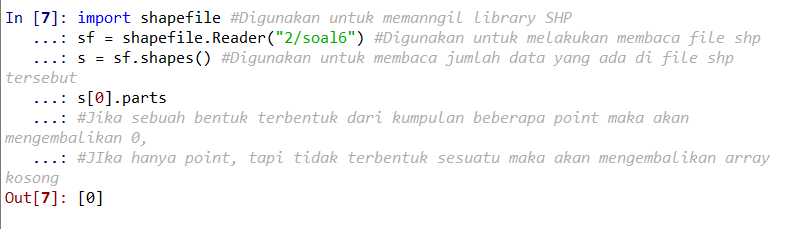
\includegraphics[width=4cm]{figures/1174021/3/soal7.PNG}
		\centering
		\caption{Hasil Read File SHP Soal 7}
    \end{figure}

    \item Buatlah Script Python dan jelaskan perbaris
    \lstinputlisting[firstline=43, lastline=47]{src/1174021/3/read.py}
    \hfill\break
     \begin{itemize}
        \item Baris pertama Digunakan untuk memanggil library SHP
        \item Digunakan untuk melakukan membaca file shp
        \item Digunakan untuk membaca jumlah data yang ada di file shp tersebut
        \item Menampilkan Koordinat yang ada pada baris tersebut
    \end{itemize}  
    \hfill\break
    \begin{figure}[H]
		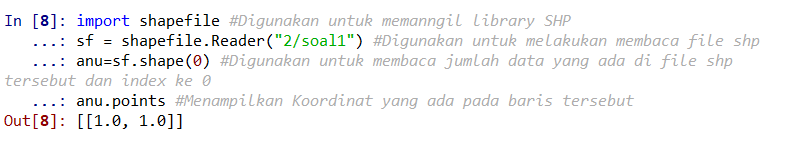
\includegraphics[width=4cm]{figures/1174021/3/soal8.PNG}
		\centering
		\caption{Hasil Read File SHP Soal 8}
    \end{figure}

    \item Buatlah Script Python dan jelaskan perbaris
    \lstinputlisting[firstline=49, lastline=53]{src/1174021/3/read.py}
    \hfill\break
    \begin{itemize}
        \item Baris pertama Digunakan untuk memanggil library SHP
        \item Digunakan untuk melakukan membaca file shp
        \item Digunakan untuk membca field yang ada pada file SHP Tersebut
        \item Digunakan Untuk menampilkan field tersebut
    \end{itemize}  
    \hfill\break
    \begin{figure}[H]
		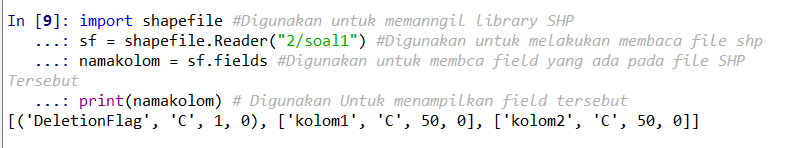
\includegraphics[width=4cm]{figures/1174021/3/soal9.PNG}
		\centering
		\caption{Hasil Read File SHP Soal 9}
    \end{figure}

    \item Buatlah Script Python dan jelaskan perbaris
    \lstinputlisting[firstline=55, lastline=59]{src/1174021/3/read.py}
    \hfill\break
    \begin{itemize}
        \item Baris pertama Digunakan untuk memanggil library SHP
        \item Digunakan untuk melakukan membaca file shp
        \item Berfungsi untuk membaca seluruh data yang ada di dalam file shp tersebut
        \item Berfungsi untuk menampilkan data tersebut
    \end{itemize}  
    \hfill\break
    \begin{figure}[H]
		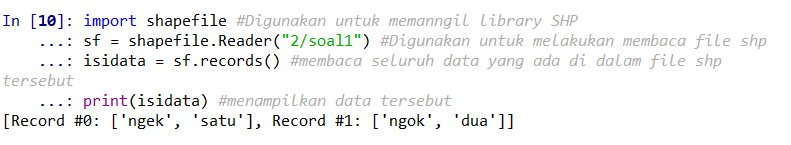
\includegraphics[width=4cm]{figures/1174021/3/soal10.PNG}
		\centering
		\caption{Hasil Read File SHP Soal 10}
    \end{figure}

    \item Buatlah Script Python dan jelaskan perbaris
    \lstinputlisting[firstline=61, lastline=66]{src/1174021/3/read.py}
    \hfill\break
    \begin{itemize}
        \item Baris pertama Digunakan untuk memanggil library SHP
        \item Digunakan untuk melakukan membaca file shp
        \item Berfungsi untuk membaca seluruh data yang ada di dalam file shp tersebut
        \item Berfungsi untuk menampilkan data pada index ke 0
        \item Berfungsi untuk menampilkan data pada index ke 0 dan urutan ke 0
    \end{itemize}  
    \hfill\break
    \begin{figure}[H]
        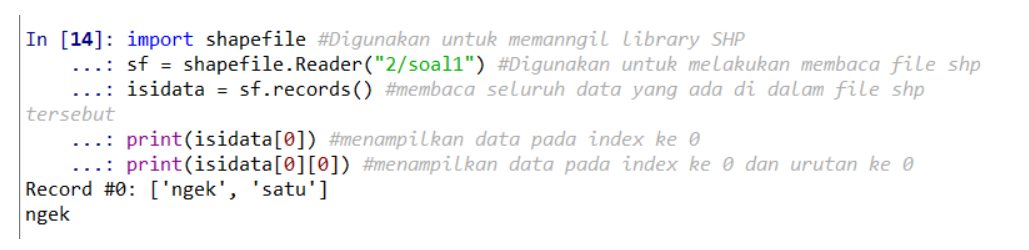
\includegraphics[width=4cm]{figures/1174021/3/soal11.PNG}
        \centering
        \caption{Hasil Read File SHP Soal 11}
    \end{figure}
\end{enumerate}

\subsection{Link Youtube}
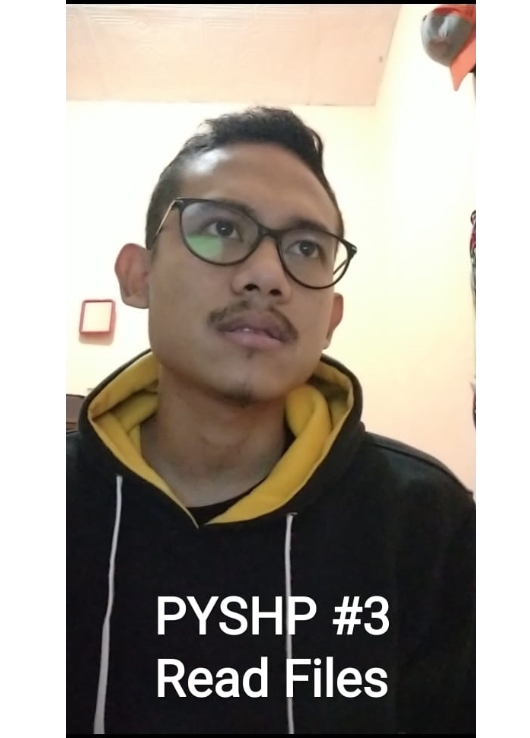
\includegraphics[width=4cm]{figures/1174021/3/fahmi3.PNG}
\href{https://youtu.be/9gqdt2JEr_E}{Video Youtube}

\subsection{Plagiarism}
\begin{figure}[H]
	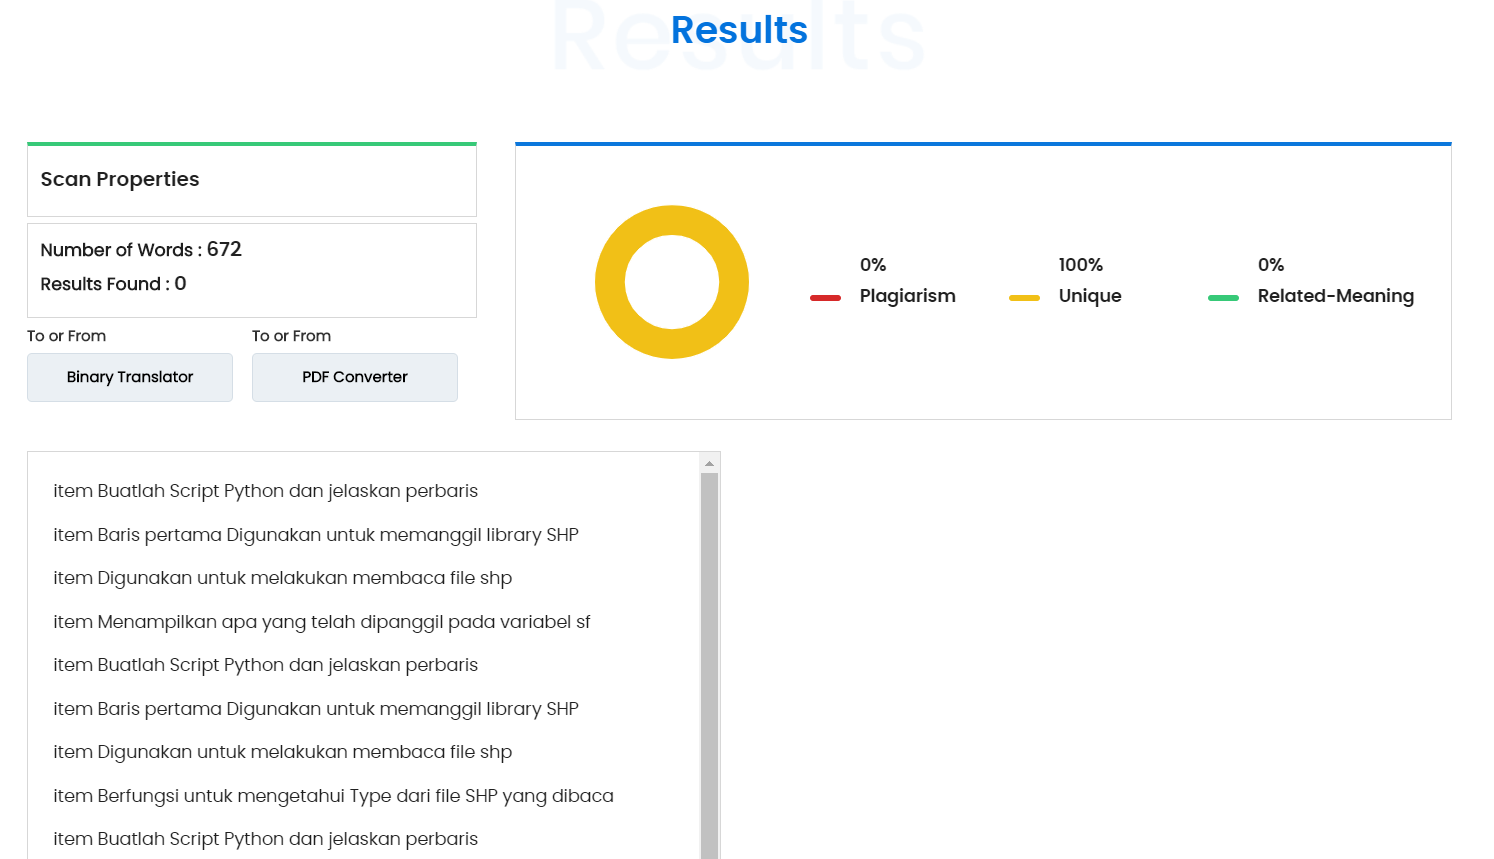
\includegraphics[width=4cm]{figures/1174021/3/buktiplagi1.PNG}
\end{figure}